
\RequirePackage{xcolor}
\documentclass[
%pdf,
%nocolorBG,
%colorBG,
%slideColor,
%slideBW,
%draft,
%frames
%azure
%contemporain
%nuancegris
%troispoints
%lignesbleues
%darkblue
%alienglow
%autumn
]{prosper}
%]{powerdot}


%\usepackage[utf8]{inputenc}
%\usepackage[T1, T2A]{fontenc}
%\usepackage[german, russian]{babel} 

\usepackage{amsmath}
%\usepackage[dvips]{color}
\usepackage{graphicx}
\usepackage{epic}
\usepackage{eepic}
%\usepackage{DBmacros}
%\usepackage{german}
%\usepackage{join}
%\usepackage{marvosym}
\usepackage{stmaryrd}
\usepackage{eurosym}
\usepackage{moresize}
\usepackage{xcolor}

%\usepackage[algo2e,vlined,linesnumbered]{algorithm2e}
%\usepackage[ruled,vlined]{algorithm2e}

\usepackage[algo2e,vlined]{algorithm2e}


%\usepackage{tikz}
%\usetikzlibrary{shadows,fadings,shadows.blur}


\definecolor{red}{rgb}{1,0,0}
\definecolor{blue}{rgb}{0,0,1}
\definecolor{white}{rgb}{1,1,1}


\include{fmakros}


\title{\textcolor{blue}{Agentic Coding}}
\author{Sven Helmer \\ Kathrin Paschen}


\begin{document}

\maketitle


%%%%%%%%%%%%%%%%%%%%%%%%%%%%%%%%%%%%%%%%%%%%%%%%%%%%%%%%%%%%%%%%%%%%%%%


\begin{slide}{Chapter 1}

\vspace*{2cm}

\begin{center}
\begin{Huge}
Introduction
\end{Huge}
\end{center}

\end{slide}




\begin{slide}{Motivation}

\begin{itemize}

\item There's a lot of hype around vibe coding at the moment

\end{itemize}


\begin{quote}
``No more humans coding in 5 years.''
\end{quote}
\hfill Emad Mostaque

\begin{quote}
``AI will write most of the code soon and perform better than top coders.''
\end{quote}
\hfill Mark Zuckerberg

\begin{quote}
``It's our job to create computing technology such that nobody has to program.''
\end{quote}
\hfill Jensen Huang


\end{slide}



\begin{slide}{Motivation (2)}

\begin{itemize}

\item We have a slightly different opinion

\item This is not the first hype we have seen

\end{itemize}

\begin{center}
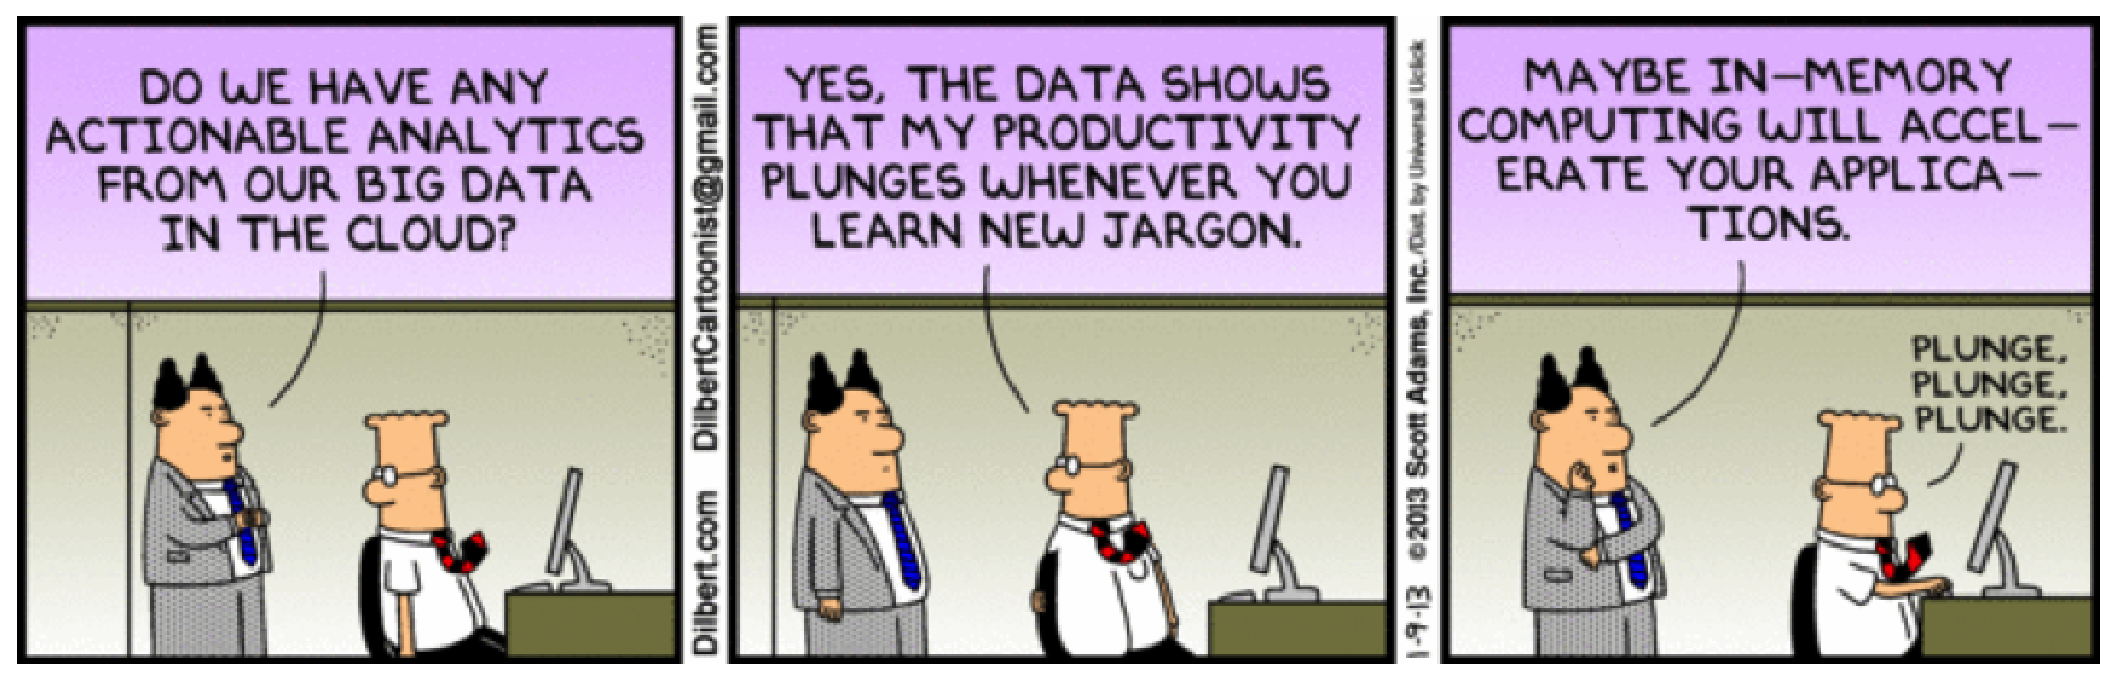
\includegraphics[width=11cm]{pics/dilbertbigdata.eps}
\end{center}

\begin{itemize}

\item We will try to bring some substance to this discussion

\end{itemize}

% comment: video dbs/datascience.mkv

\end{slide}




\begin{slide}{Things are Definitely Changing}

\begin{itemize}

\item In the foreseeable future, AI will not replace developers

\begin{itemize}
  
\item A developer using AI will replace one who doesn't

\item and developers (already) work differently
  
\end{itemize}
  
\item Currently, AI boosts the skills of experienced experts

\item It will not save you if you have no clue what you're doing

\end{itemize}

\end{slide}




\begin{slide}{Basic Terminology}

\begin{itemize}

\item Coding with AI covers a whole spectrum
 
\begin{itemize}

\item Vibe coding: prompt and hope for the best

\item Agentic coding: a systematic approach that still utilizes software
  development principles

\end{itemize}

\end{itemize}

\vspace*{.5cm}
\begin{center}
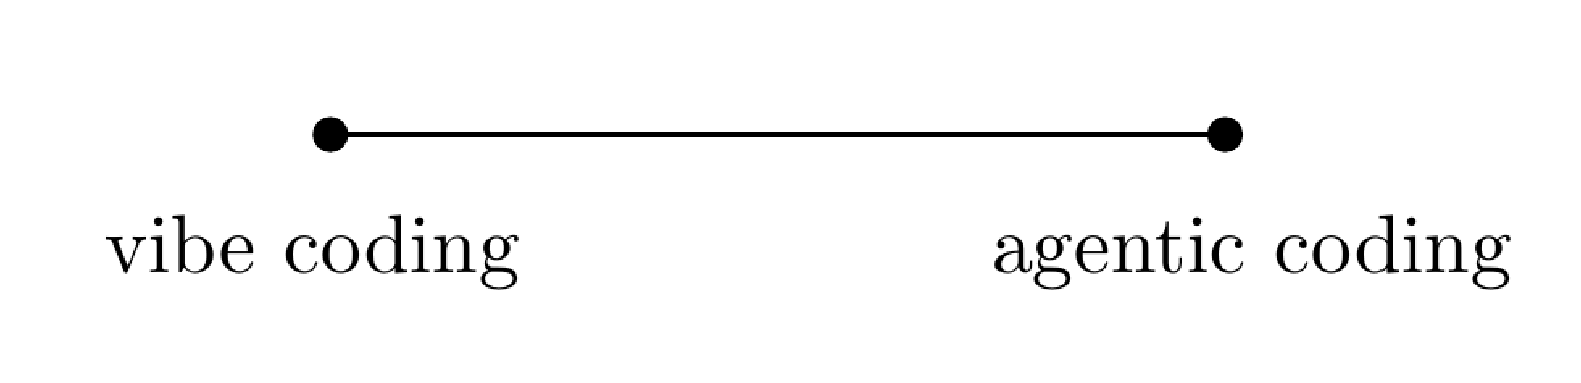
\includegraphics[width=8cm]{pics/vibevsagentic.eps}
\end{center}

\end{slide}




\begin{slide}{Vibe Coding}

\begin{itemize}

\item Vibe coding typically looks like the following:

\begin{itemize}

\item Write a prompt, e.g. ``Build an app that does X.''

\item LLM generates some code

\item User tries it out, doesn't quite work

\item User writes another prompt requesting some changes

\item LLM changes code

\item Wash, rinse, repeat

\end{itemize}
  

\end{itemize}
  
\end{slide}



\begin{slide}{Agentic Coding}

\begin{itemize}

\item This is not about writing simple prompts

\item Gives an LLM specific software development tasks in a systematic way,
  such as:

\begin{itemize}

\item Formulate goal, e.g., in form of a specification

\item Devise a plan, break up general task into subtasks

\item Generate code

\item Validate code, e.g., by running tests

\item If necessary, revise implementation (or even planning)

\end{itemize}

\end{itemize}
  
\end{slide}



\begin{slide}{Vibe-Coding vs. Agentic Coding}

\begin{itemize}

\item That doesn't necessarily mean that vibe coding is bad and agentic coding
  is good

\item Vibe coding:

  \begin{itemize}
    
  \item makes sense for rapid prototyping
    
  \item is for quickly trying out things
    
  \end{itemize}
    
\item Agentic coding

  \begin{itemize}
    
  \item is a thorough process
    
  \item creates reliable code
    
  \end{itemize}

\end{itemize}
  
\end{slide}



\begin{slide}{What Can Go Wrong?}

\begin{itemize}

\item AI gets stuck in infinite loops

\item Deliver incorrect solutions confidently

\item Cheat: optimize for validation such as benchmarks
  
\item Implements what you said, not what you meant

\begin{itemize}

\item General problem, existed before AI

\end{itemize}
  
\end{itemize}
  
\end{slide}



\begin{slide}{Summary}

\begin{itemize}

\item Then: translate ideas into code (programming)

\item Now: translate ideas into prompts (vibe-coding)

\item Then: (systematically) applying principles and methods to create
  reliable software (software engineering)

\item Now: give an AI (software-engineering) goals and constraints to create
  software (agentic coding)

\item Important question: how much of the software-engineering process can be
  delegated?
  
  
\end{itemize}
  
\end{slide}



\begin{slide}{}

\begin{itemize}

\item 

\end{itemize}
  
\end{slide}



\begin{slide}{}

\begin{itemize}

\item 

\end{itemize}
  
\end{slide}



\begin{slide}{}

\begin{itemize}

\item 

\end{itemize}
  
\end{slide}



\begin{slide}{}

\begin{itemize}

\item 

\end{itemize}
  
\end{slide}



\begin{slide}{}

\begin{itemize}

\item 

\end{itemize}
  
\end{slide}







%%%%%%%%%%%%%%%%%%%%%%%%%%%%%%%%%%%%%%%%%%%%%%%%%%%%%%%%%%%%%%%%%%%%%%%





\end{document}




\begin{slide}{Chapter 2}

\vspace*{2cm}

\begin{center}
\begin{Huge}
xxx
\end{Huge}
\end{center}

\end{slide}




\begin{slide}{}

\begin{itemize}

\item 

\end{itemize}
  
\end{slide}



\begin{slide}{}

\begin{itemize}

\item 

\end{itemize}
  
\end{slide}



\begin{slide}{}

\begin{itemize}

\item 

\end{itemize}
  
\end{slide}



